% Options for packages loaded elsewhere
\PassOptionsToPackage{unicode}{hyperref}
\PassOptionsToPackage{hyphens}{url}
%
\documentclass[
]{article}
\usepackage{amsmath,amssymb}
\usepackage{lmodern}
\usepackage{ifxetex,ifluatex}
\ifnum 0\ifxetex 1\fi\ifluatex 1\fi=0 % if pdftex
  \usepackage[T1]{fontenc}
  \usepackage[utf8]{inputenc}
  \usepackage{textcomp} % provide euro and other symbols
\else % if luatex or xetex
  \usepackage{unicode-math}
  \defaultfontfeatures{Scale=MatchLowercase}
  \defaultfontfeatures[\rmfamily]{Ligatures=TeX,Scale=1}
\fi
% Use upquote if available, for straight quotes in verbatim environments
\IfFileExists{upquote.sty}{\usepackage{upquote}}{}
\IfFileExists{microtype.sty}{% use microtype if available
  \usepackage[]{microtype}
  \UseMicrotypeSet[protrusion]{basicmath} % disable protrusion for tt fonts
}{}
\makeatletter
\@ifundefined{KOMAClassName}{% if non-KOMA class
  \IfFileExists{parskip.sty}{%
    \usepackage{parskip}
  }{% else
    \setlength{\parindent}{0pt}
    \setlength{\parskip}{6pt plus 2pt minus 1pt}}
}{% if KOMA class
  \KOMAoptions{parskip=half}}
\makeatother
\usepackage{xcolor}
\IfFileExists{xurl.sty}{\usepackage{xurl}}{} % add URL line breaks if available
\IfFileExists{bookmark.sty}{\usepackage{bookmark}}{\usepackage{hyperref}}
\hypersetup{
  pdftitle={Using HTML Comments to Facilitate Colaboration with Git},
  pdfauthor={R. Mark Sharp},
  hidelinks,
  pdfcreator={LaTeX via pandoc}}
\urlstyle{same} % disable monospaced font for URLs
\usepackage[margin=1in]{geometry}
\usepackage{color}
\usepackage{fancyvrb}
\newcommand{\VerbBar}{|}
\newcommand{\VERB}{\Verb[commandchars=\\\{\}]}
\DefineVerbatimEnvironment{Highlighting}{Verbatim}{commandchars=\\\{\}}
% Add ',fontsize=\small' for more characters per line
\usepackage{framed}
\definecolor{shadecolor}{RGB}{248,248,248}
\newenvironment{Shaded}{\begin{snugshade}}{\end{snugshade}}
\newcommand{\AlertTok}[1]{\textcolor[rgb]{0.94,0.16,0.16}{#1}}
\newcommand{\AnnotationTok}[1]{\textcolor[rgb]{0.56,0.35,0.01}{\textbf{\textit{#1}}}}
\newcommand{\AttributeTok}[1]{\textcolor[rgb]{0.77,0.63,0.00}{#1}}
\newcommand{\BaseNTok}[1]{\textcolor[rgb]{0.00,0.00,0.81}{#1}}
\newcommand{\BuiltInTok}[1]{#1}
\newcommand{\CharTok}[1]{\textcolor[rgb]{0.31,0.60,0.02}{#1}}
\newcommand{\CommentTok}[1]{\textcolor[rgb]{0.56,0.35,0.01}{\textit{#1}}}
\newcommand{\CommentVarTok}[1]{\textcolor[rgb]{0.56,0.35,0.01}{\textbf{\textit{#1}}}}
\newcommand{\ConstantTok}[1]{\textcolor[rgb]{0.00,0.00,0.00}{#1}}
\newcommand{\ControlFlowTok}[1]{\textcolor[rgb]{0.13,0.29,0.53}{\textbf{#1}}}
\newcommand{\DataTypeTok}[1]{\textcolor[rgb]{0.13,0.29,0.53}{#1}}
\newcommand{\DecValTok}[1]{\textcolor[rgb]{0.00,0.00,0.81}{#1}}
\newcommand{\DocumentationTok}[1]{\textcolor[rgb]{0.56,0.35,0.01}{\textbf{\textit{#1}}}}
\newcommand{\ErrorTok}[1]{\textcolor[rgb]{0.64,0.00,0.00}{\textbf{#1}}}
\newcommand{\ExtensionTok}[1]{#1}
\newcommand{\FloatTok}[1]{\textcolor[rgb]{0.00,0.00,0.81}{#1}}
\newcommand{\FunctionTok}[1]{\textcolor[rgb]{0.00,0.00,0.00}{#1}}
\newcommand{\ImportTok}[1]{#1}
\newcommand{\InformationTok}[1]{\textcolor[rgb]{0.56,0.35,0.01}{\textbf{\textit{#1}}}}
\newcommand{\KeywordTok}[1]{\textcolor[rgb]{0.13,0.29,0.53}{\textbf{#1}}}
\newcommand{\NormalTok}[1]{#1}
\newcommand{\OperatorTok}[1]{\textcolor[rgb]{0.81,0.36,0.00}{\textbf{#1}}}
\newcommand{\OtherTok}[1]{\textcolor[rgb]{0.56,0.35,0.01}{#1}}
\newcommand{\PreprocessorTok}[1]{\textcolor[rgb]{0.56,0.35,0.01}{\textit{#1}}}
\newcommand{\RegionMarkerTok}[1]{#1}
\newcommand{\SpecialCharTok}[1]{\textcolor[rgb]{0.00,0.00,0.00}{#1}}
\newcommand{\SpecialStringTok}[1]{\textcolor[rgb]{0.31,0.60,0.02}{#1}}
\newcommand{\StringTok}[1]{\textcolor[rgb]{0.31,0.60,0.02}{#1}}
\newcommand{\VariableTok}[1]{\textcolor[rgb]{0.00,0.00,0.00}{#1}}
\newcommand{\VerbatimStringTok}[1]{\textcolor[rgb]{0.31,0.60,0.02}{#1}}
\newcommand{\WarningTok}[1]{\textcolor[rgb]{0.56,0.35,0.01}{\textbf{\textit{#1}}}}
\usepackage{graphicx}
\makeatletter
\def\maxwidth{\ifdim\Gin@nat@width>\linewidth\linewidth\else\Gin@nat@width\fi}
\def\maxheight{\ifdim\Gin@nat@height>\textheight\textheight\else\Gin@nat@height\fi}
\makeatother
% Scale images if necessary, so that they will not overflow the page
% margins by default, and it is still possible to overwrite the defaults
% using explicit options in \includegraphics[width, height, ...]{}
\setkeys{Gin}{width=\maxwidth,height=\maxheight,keepaspectratio}
% Set default figure placement to htbp
\makeatletter
\def\fps@figure{htbp}
\makeatother
\setlength{\emergencystretch}{3em} % prevent overfull lines
\providecommand{\tightlist}{%
  \setlength{\itemsep}{0pt}\setlength{\parskip}{0pt}}
\setcounter{secnumdepth}{-\maxdimen} % remove section numbering
\usepackage{booktabs}
\usepackage{longtable}
\usepackage{array}
\usepackage{multirow}
\usepackage{wrapfig}
\usepackage{float}
\usepackage{colortbl}
\usepackage{pdflscape}
\usepackage{tabu}
\usepackage{threeparttable}
\usepackage{threeparttablex}
\usepackage[normalem]{ulem}
\usepackage{makecell}
\usepackage{xcolor}
\ifluatex
  \usepackage{selnolig}  % disable illegal ligatures
\fi

\title{Using HTML Comments to Facilitate Colaboration with Git}
\author{R. Mark Sharp}
\date{2021-03-08}

\begin{document}
\maketitle

{
\setcounter{tocdepth}{2}
\tableofcontents
}
\hypertarget{introduction}{%
\subsection{Introduction}\label{introduction}}

Retention of collaborative interactions that appear as back and forth
comments within source documents of a project is a valuable source of
history and subsequent education and process improvement. However, it is
often the case that at the end of the development phase those
interactions need to be removed before sending the source files to
further review or production. This tutorial provides one method and a
set of tools to both collaborate via HTML comments and remove comments
selectively when needed.

\hypertarget{collaboration}{%
\subsection{Collaboration}\label{collaboration}}

HTML comments can be inserted into an RMarkdown document as a means of
communicating with others or making a note to yourself. The workflow
illustrated herein uses a text label immediately after the beginning
characters of the HTML comment (i.e., \texttt{\textless{}!-\/-}). White
space, including blank lines are ignored. Thus, any of the following
will be seen as a comment.

\begin{Shaded}
\begin{Highlighting}[]
\StringTok{\textasciigrave{}}\AttributeTok{\textless{}!{-}{-} This is a comment without a useful label {-}{-}\textgreater{}}\StringTok{\textasciigrave{}}
\StringTok{\textasciigrave{}}\AttributeTok{\textless{}!{-}{-} RMS This is a one line comment that has my intitials as its label.{-}{-}\textgreater{}}\StringTok{\textasciigrave{}}
\StringTok{\textasciigrave{}}\AttributeTok{\textless{}!{-}{-}}
\AttributeTok{RMS Comments can span multiple lines and later can be entirely removed by}
\AttributeTok{either selecting to remove all comments or only those comments that have}
\AttributeTok{labels you provide as a character vector to the "label" parameter}
\AttributeTok{{-}{-}\textgreater{}}\StringTok{\textasciigrave{}}
\end{Highlighting}
\end{Shaded}

Collaboration will usually involve suggestions and perhaps corrections.

\begin{Shaded}
\begin{Highlighting}[]
  \FunctionTok{xt\_print}\NormalTok{(all\_unusual\_wts\_sex,}
           \AttributeTok{caption =} \FunctionTok{stri\_c}\NormalTok{(common\_name, }\StringTok{":  "}\NormalTok{, animal\_count, }\StringTok{" "}\NormalTok{, sex\_str,}
                           \StringTok{" with weights outside the "}\NormalTok{,}
                           \FunctionTok{signif}\NormalTok{(conf\_int }\SpecialCharTok{*} \DecValTok{100}\NormalTok{, }\DecValTok{3}\NormalTok{),}
                           \StringTok{"}\SpecialCharTok{\textbackslash{}\textbackslash{}}\StringTok{\% predicted range."}\NormalTok{),}
           \AttributeTok{label =} \FunctionTok{stri\_c}\NormalTok{(}\StringTok{"tbl:"}\NormalTok{, arc\_species\_code, }\StringTok{"{-}"}\NormalTok{, sex),}
           \AttributeTok{format.args =} \FunctionTok{list}\NormalTok{(}\AttributeTok{big.mark =} \StringTok{","}\NormalTok{, }\AttributeTok{decimal.mark =} \StringTok{"."}\NormalTok{),}
           \AttributeTok{size =}\NormalTok{ size)}

\StringTok{\textasciigrave{}}\AttributeTok{\textless{}!{-}{-} RMS I added some formating code (format.args) in the call to xt\_print}
\AttributeTok{     please look at the output to see whether or not you prefer that formating}
\AttributeTok{     decision.{-}{-}\textgreater{}}\StringTok{\textasciigrave{}}
\end{Highlighting}
\end{Shaded}

The collaborator (TJH) can add his own comment or add to the original to
inform RMS that the change was considered.

\begin{Shaded}
\begin{Highlighting}[]
\StringTok{\textasciigrave{}}\AttributeTok{\textless{}!{-}{-} RMS I added some formating code (format.args) in the call to xt\_print}
\AttributeTok{     please look at the output to see whether or not you prefer that formating}
\AttributeTok{     decision.}
\AttributeTok{     *** TJH I like the change as some of the numbers are over 10\^{}5}
\AttributeTok{ {-}{-}\textgreater{}}\StringTok{\textasciigrave{}}
\end{Highlighting}
\end{Shaded}

Alternatively, TJH may decide to keep his response separate from the
original comment by adding his own separate comment.

\begin{Shaded}
\begin{Highlighting}[]
\StringTok{\textasciigrave{}}\AttributeTok{\textless{}!{-}{-} RMS I added some formating code (format.args) in the call to xt\_print}
\AttributeTok{     please look at the output to see whether or not you prefer that formating}
\AttributeTok{     decision.}
\AttributeTok{ {-}{-}\textgreater{}}\StringTok{\textasciigrave{}}
\StringTok{\textasciigrave{}}\AttributeTok{\textless{}!{-}{-} TJH I like the change as some of the numbers are over 10\^{}5}
\AttributeTok{ {-}{-}\textgreater{}}\StringTok{\textasciigrave{}}
\end{Highlighting}
\end{Shaded}

We recommend the first convention as it keeps related comments together
and still allows identification of participants within the conversation.

Later, reasons for selecting one convention over the other will be
discussed again when removal of comments is described.

\hypertarget{review}{%
\subsection{Review}\label{review}}

HTML comments can also be used as a part of a review process. This is
not conceptually different that other forms of collaboration but the
need to indicate acceptance or rejection of suggestions and final
approval is demonstrated in the following versions of text.

\begin{Shaded}
\begin{Highlighting}[]
  \FunctionTok{xt\_print}\NormalTok{(bad\_sample\_dates\_df, }\AttributeTok{caption =} \StringTok{"Bad Sample Dates"}\NormalTok{,}
           \AttributeTok{label =} \StringTok{"tbl:bad{-}sample{-}dates"}\NormalTok{, }\AttributeTok{type =}\NormalTok{ type, ...)}
  

\StringTok{\textasciigrave{}}\AttributeTok{\textless{}!{-}{-} RMS The caption reads like a title. Consider using a caption that allows}
\AttributeTok{the table to be understood without forcing the reader to go find the }
\AttributeTok{narrative that describes the table contents.}
\AttributeTok{{-}{-}\textgreater{}}\StringTok{\textasciigrave{}}
\end{Highlighting}
\end{Shaded}

The document author can respond to the request by simply editing the
code. However, editing to comment allows the review to quickly see that
the concern was acknowledged and addressed.

\begin{Shaded}
\begin{Highlighting}[]
    \ControlFlowTok{if}\NormalTok{ (}\FunctionTok{nrow}\NormalTok{(bad\_sample\_dates\_df) }\SpecialCharTok{==} \DecValTok{1}\NormalTok{) \{}
\NormalTok{      caption }\OtherTok{\textless{}{-}} \FunctionTok{stri\_c}\NormalTok{(}
        \StringTok{"There was 1 bad sample date identified where the animal was not}
\StringTok{        present on the date indicated."}\NormalTok{)}
\NormalTok{    \} }\ControlFlowTok{else}\NormalTok{ \{}
\NormalTok{      caption }\OtherTok{\textless{}{-}} \FunctionTok{stri\_c}\NormalTok{(}
        \StringTok{"There were "}\NormalTok{, }\FunctionTok{nrow}\NormalTok{(bad\_sample\_dates\_df), }\StringTok{" bad sample dates identified}
\StringTok{        where the animals were not present on the dates indicated."}\NormalTok{)}
\NormalTok{    \}}

    \FunctionTok{xt\_print}\NormalTok{(bad\_sample\_dates\_df, }\AttributeTok{caption =}\NormalTok{ caption,}
             \AttributeTok{label =} \StringTok{"tbl:bad{-}sample{-}dates"}\NormalTok{, }\AttributeTok{type =}\NormalTok{ type, ...)}
  


\StringTok{\textasciigrave{}}\AttributeTok{\textless{}!{-}{-} RMS The caption reads like a title. Consider using a caption that allows}
\AttributeTok{the table to be understood without forcing the reader to go find the }
\AttributeTok{narrative that describes the table contents.}
\AttributeTok{*** TJH I added a more helpful dynamically generated caption so that the text }
\AttributeTok{reflects the number of bad dates shown.}
\AttributeTok{{-}{-}\textgreater{}}\StringTok{\textasciigrave{}}
\end{Highlighting}
\end{Shaded}

The reviewer can then note that the change was seen and accepted.

\begin{Shaded}
\begin{Highlighting}[]
\StringTok{\textasciigrave{}}\AttributeTok{\textless{}!{-}{-} RMS The caption reads like a title. Consider using a caption that allows}
\AttributeTok{the table to be understood without forcing the reader to go find the }
\AttributeTok{narrative that describes the table contents.}
\AttributeTok{*** TJH I added a more helpful dynamically generated caption so that the text }
\AttributeTok{reflects the number of bad dates shown.}
\AttributeTok{*** RMS Nicely done. I like the dynamically generated caption.}
\AttributeTok{accepted 20210215}
\AttributeTok{{-}{-}\textgreater{}}\StringTok{\textasciigrave{}}
\end{Highlighting}
\end{Shaded}

\hypertarget{locating-comments}{%
\subsection{Locating Comments}\label{locating-comments}}

Retention of comments during the document development phase is helpful
so that decisions made earlier are not forgotten with the result of time
being wasted rethinking earlier topics of discussion.

There are several functions that can be used to produce various
inventories of HTML comments within RMarkdown source files.

\begin{itemize}
\tightlist
\item
  \textbf{get\_html\_comment\_text\_lines\_and\_labels\_from\_files}
\end{itemize}

Takes a vector of files\footnote{This example uses a single file,
  however, multiple files with fully qualified file names in the
  character vector is expected.} and labels to retrieve and returns a
dataframe with full file paths, the base file names, starting line
number of each comment, the end line number of each comment, and the
identifying labels. This dataframe is ordered by path, label, and
starting line number of the comment.

The default value of the \texttt{label} argument is \texttt{""} when no
definition is provided.

\begin{Shaded}
\begin{Highlighting}[]
\NormalTok{files }\OtherTok{=} \FunctionTok{system.file}\NormalTok{(}\StringTok{"testdata"}\NormalTok{,}\StringTok{"find\_html\_comment\_test\_file.Rmd"}\NormalTok{, }
                       \AttributeTok{package =} \StringTok{"rmsutilityr"}\NormalTok{)}
\NormalTok{html\_comment\_lines\_and\_labels }\OtherTok{\textless{}{-}} 
  \FunctionTok{get\_html\_comment\_text\_lines\_and\_labels\_from\_files}\NormalTok{(files)}

\NormalTok{caption }\OtherTok{\textless{}{-}} 
\NormalTok{  knitr}\SpecialCharTok{:::}\FunctionTok{escape\_latex}\NormalTok{(}\FunctionTok{stri\_c}\NormalTok{(}\StringTok{"Output of the "}\NormalTok{, }
         \StringTok{"get\_html\_comment\_text\_lines\_and\_labels\_from\_files "}\NormalTok{,}
         \StringTok{"function includes all comments when no \textquotesingle{}label\textquotesingle{} parameter is "}\NormalTok{, }
         \StringTok{"provided. The columns include the file name (no path), "}\NormalTok{,}
         \StringTok{"the possible label, the line number where the comment "}\NormalTok{,}
         \StringTok{"starts, and the line number where the comment ends."}\NormalTok{))}


 \FunctionTok{kbl}\NormalTok{(html\_comment\_lines\_and\_labels[ , }\FunctionTok{c}\NormalTok{(}\StringTok{"file"}\NormalTok{, }\StringTok{"comment\_label"}\NormalTok{, }
                                            \StringTok{"comment\_start\_line"}\NormalTok{, }
                                            \StringTok{"comment\_end\_line"}\NormalTok{)],}
     \AttributeTok{format =} \FunctionTok{ifelse}\NormalTok{(knitr}\SpecialCharTok{::}\FunctionTok{is\_latex\_output}\NormalTok{(), }\StringTok{"latex"}\NormalTok{, }\StringTok{"html"}\NormalTok{),}
     \AttributeTok{longtable =} \ConstantTok{TRUE}\NormalTok{, }\AttributeTok{booktabs =} \ConstantTok{TRUE}\NormalTok{,}
     \AttributeTok{caption =}\NormalTok{ caption,}
     \AttributeTok{row.names =} \ConstantTok{FALSE}\NormalTok{,}
     \AttributeTok{col.names =} \FunctionTok{c}\NormalTok{(}\StringTok{"File"}\NormalTok{, }\StringTok{"Label"}\NormalTok{, }\StringTok{"Start"}\NormalTok{, }\StringTok{"End"}\NormalTok{)) }\SpecialCharTok{\%\textgreater{}\%}
   \FunctionTok{kable\_styling}\NormalTok{(}\AttributeTok{latex\_options =} \FunctionTok{c}\NormalTok{(}\StringTok{"repeat\_header"}\NormalTok{, }\StringTok{"striped"}\NormalTok{), }
                 \AttributeTok{font\_size =} \FunctionTok{ifelse}\NormalTok{(knitr}\SpecialCharTok{::}\FunctionTok{is\_latex\_output}\NormalTok{(), }\DecValTok{8}\NormalTok{, }\DecValTok{12}\NormalTok{))}
\end{Highlighting}
\end{Shaded}

\begingroup\fontsize{8}{10}\selectfont

\begin{longtable}[t]{llrr}
\caption{\label{tab:get-all-comments-from-file}Output of the get\_html\_comment\_text\_lines\_and\_labels\_from\_files function includes all comments when no 'label' parameter is provided. The columns include the file name (no path), the possible label, the line number where the comment starts, and the line number where the comment ends.}\\
\toprule
File & Label & Start & End\\
\midrule
\endfirsthead
\caption[]{Output of the get\_html\_comment\_text\_lines\_and\_labels\_from\_files function includes all comments when no 'label' parameter is provided. The columns include the file name (no path), the possible label, the line number where the comment starts, and the line number where the comment ends. \textit{(continued)}}\\
\toprule
File & Label & Start & End\\
\midrule
\endhead

\endfoot
\bottomrule
\endlastfoot
\cellcolor{gray!6}{find\_html\_comment\_test\_file.Rmd} & \cellcolor{gray!6}{I} & \cellcolor{gray!6}{26} & \cellcolor{gray!6}{26}\\
find\_html\_comment\_test\_file.Rmd & RMS & 16 & 18\\
\cellcolor{gray!6}{find\_html\_comment\_test\_file.Rmd} & \cellcolor{gray!6}{RMS} & \cellcolor{gray!6}{30} & \cellcolor{gray!6}{32}\\
find\_html\_comment\_test\_file.Rmd & RMS & 34 & 35\\
\cellcolor{gray!6}{find\_html\_comment\_test\_file.Rmd} & \cellcolor{gray!6}{SRR} & \cellcolor{gray!6}{25} & \cellcolor{gray!6}{25}\\
\addlinespace
find\_html\_comment\_test\_file.Rmd & TJH & 22 & 23\\*
\end{longtable}
\endgroup{}

This same function can be used to review the text of comments from
selected collaborators.

\begin{Shaded}
\begin{Highlighting}[]
\NormalTok{files }\OtherTok{=} \FunctionTok{system.file}\NormalTok{(}\StringTok{"testdata"}\NormalTok{,}\StringTok{"find\_html\_comment\_test\_file.Rmd"}\NormalTok{, }
                       \AttributeTok{package =} \StringTok{"rmsutilityr"}\NormalTok{)}
\NormalTok{html\_comment\_lines\_and\_labels }\OtherTok{\textless{}{-}} 
  \FunctionTok{get\_html\_comment\_text\_lines\_and\_labels\_from\_files}\NormalTok{(files, }\AttributeTok{label =} \StringTok{"RMS"}\NormalTok{)}

\NormalTok{caption }\OtherTok{\textless{}{-}} 
\NormalTok{  knitr}\SpecialCharTok{:::}\FunctionTok{escape\_latex}\NormalTok{(}\FunctionTok{stri\_c}\NormalTok{(}\StringTok{"Output of the "}\NormalTok{, }
         \StringTok{"get\_html\_comment\_text\_lines\_and\_labels\_from\_files "}\NormalTok{,}
         \StringTok{"function includes text of comments from selected "}\NormalTok{,}
         \StringTok{"comment labels."}\NormalTok{))}


 \FunctionTok{kbl}\NormalTok{(html\_comment\_lines\_and\_labels[ , }\FunctionTok{c}\NormalTok{(}\StringTok{"file"}\NormalTok{, }\StringTok{"comment\_label"}\NormalTok{,}
                                        \StringTok{"comment\_start\_line"}\NormalTok{,}
                                        \StringTok{"comment\_text"}\NormalTok{)],}
     \AttributeTok{format =} \FunctionTok{ifelse}\NormalTok{(knitr}\SpecialCharTok{::}\FunctionTok{is\_latex\_output}\NormalTok{(), }\StringTok{"latex"}\NormalTok{, }\StringTok{"html"}\NormalTok{),}
     \AttributeTok{booktabs =} \ConstantTok{TRUE}\NormalTok{, }\AttributeTok{caption =}\NormalTok{ caption,}
     \AttributeTok{row.names =} \ConstantTok{FALSE}\NormalTok{,}
     \AttributeTok{col.names =} \FunctionTok{c}\NormalTok{(}\StringTok{"File"}\NormalTok{, }\StringTok{"Label"}\NormalTok{, }\StringTok{"Start"}\NormalTok{, }\StringTok{"Text"}\NormalTok{),}
     \AttributeTok{longtable =} \ConstantTok{TRUE}\NormalTok{) }\SpecialCharTok{\%\textgreater{}\%} 
   \FunctionTok{kable\_styling}\NormalTok{(}\AttributeTok{latex\_options =} \FunctionTok{c}\NormalTok{(}\StringTok{"repeat\_header"}\NormalTok{, }\StringTok{"striped"}\NormalTok{), }
                 \AttributeTok{font\_size =} \FunctionTok{ifelse}\NormalTok{(knitr}\SpecialCharTok{::}\FunctionTok{is\_latex\_output}\NormalTok{(), }\DecValTok{8}\NormalTok{, }\DecValTok{12}\NormalTok{)) }\SpecialCharTok{\%\textgreater{}\%}
   \FunctionTok{column\_spec}\NormalTok{(}\DecValTok{1}\NormalTok{, }\AttributeTok{width =} \StringTok{"15em"}\NormalTok{) }\SpecialCharTok{\%\textgreater{}\%}
   \FunctionTok{column\_spec}\NormalTok{(}\DecValTok{2}\NormalTok{, }\AttributeTok{width =} \StringTok{"5em"}\NormalTok{) }\SpecialCharTok{\%\textgreater{}\%}
   \FunctionTok{column\_spec}\NormalTok{(}\DecValTok{3}\NormalTok{, }\AttributeTok{width =} \StringTok{"5em"}\NormalTok{) }\SpecialCharTok{\%\textgreater{}\%}
   \FunctionTok{column\_spec}\NormalTok{(}\DecValTok{4}\NormalTok{, }\AttributeTok{width =} \StringTok{"25em"}\NormalTok{) }
\end{Highlighting}
\end{Shaded}

\begingroup\fontsize{8}{10}\selectfont

\begin{longtable}[t]{>{\raggedright\arraybackslash}p{15em}>{\raggedright\arraybackslash}p{5em}>{\raggedleft\arraybackslash}p{5em}>{\raggedright\arraybackslash}p{25em}}
\caption{\label{tab:get-selected-comment-text-from-file}Output of the get\_html\_comment\_text\_lines\_and\_labels\_from\_files function includes text of comments from selected comment labels.}\\
\toprule
File & Label & Start & Text\\
\midrule
\endfirsthead
\caption[]{Output of the get\_html\_comment\_text\_lines\_and\_labels\_from\_files function includes text of comments from selected comment labels. \textit{(continued)}}\\
\toprule
File & Label & Start & Text\\
\midrule
\endhead

\endfoot
\bottomrule
\endlastfoot
\cellcolor{gray!6}{find\_html\_comment\_test\_file.Rmd} & \cellcolor{gray!6}{RMS} & \cellcolor{gray!6}{16} & \cellcolor{gray!6}{This is a comment that I want to notice later. To help others see it, I decided to write more words than are needed.}\\
find\_html\_comment\_test\_file.Rmd & RMS & 30 & Let's count this one\\
\cellcolor{gray!6}{find\_html\_comment\_test\_file.Rmd} & \cellcolor{gray!6}{RMS} & \cellcolor{gray!6}{34} & \cellcolor{gray!6}{I am counting this too.}\\*
\end{longtable}
\endgroup{}

\hypertarget{deleting-comments}{%
\subsection{Deleting Comments}\label{deleting-comments}}

As stated earlier, in some workflows it is an advantage to remove
collaborators' and reviewers' comments from the final document to clean
up the presentation and to prevent unintended influence on subsequent
readers of the source RMarkdown document.

This can be done by providing a character vector of full or relative
path names and a directory to place the edited files in to using the
\texttt{write\_files\_after\_deleting\_selected\_comments} function.

\begin{Shaded}
\begin{Highlighting}[]
\NormalTok{files }\OtherTok{=} \FunctionTok{system.file}\NormalTok{(}\StringTok{"testdata"}\NormalTok{,}\StringTok{"find\_html\_comment\_test\_file.Rmd"}\NormalTok{, }
                   \AttributeTok{package =} \StringTok{"rmsutilityr"}\NormalTok{)}
\NormalTok{new\_files }\OtherTok{\textless{}{-}} 
  \FunctionTok{write\_files\_after\_deleting\_selected\_comments}\NormalTok{(}\AttributeTok{new\_path =} \FunctionTok{tempdir}\NormalTok{(), }
\NormalTok{                                               files, }\AttributeTok{label =} \StringTok{"RMS"}\NormalTok{)}
\NormalTok{new\_files}
\end{Highlighting}
\end{Shaded}

\begin{verbatim}
## [1] "/var/folders/y3/5z1skj6s5tq0pktmsq6x80v80000gn/T//RtmpsrkP2c/find_html_comment_test_file.Rmd"
\end{verbatim}

\hypertarget{reviewing-comments}{%
\subsection{Reviewing Comments}\label{reviewing-comments}}

\hypertarget{counting-comments}{%
\subsubsection{Counting Comments}\label{counting-comments}}

You can count comments in your files quickly with this helper
function\footnote{ A commented version of the same convenience function
  is included in this package.}

\begin{Shaded}
\begin{Highlighting}[]
\NormalTok{count\_selected\_comments }\OtherTok{\textless{}{-}} \ControlFlowTok{function}\NormalTok{(files, }\AttributeTok{label =} \StringTok{""}\NormalTok{) \{}
\NormalTok{  comment\_count }\OtherTok{\textless{}{-}} \DecValTok{0}
  \ControlFlowTok{for}\NormalTok{ (file }\ControlFlowTok{in}\NormalTok{ files) \{}
\NormalTok{    lines }\OtherTok{\textless{}{-}} \FunctionTok{readLines}\NormalTok{(file)}
\NormalTok{    lines\_and\_labels }\OtherTok{\textless{}{-}} \FunctionTok{return\_html\_comment\_text\_lines\_and\_labels}\NormalTok{(lines, label)}
\NormalTok{    comment\_count }\OtherTok{\textless{}{-}}\NormalTok{ comment\_count }\SpecialCharTok{+} \FunctionTok{length}\NormalTok{(lines\_and\_labels[[}\DecValTok{1}\NormalTok{]])}
\NormalTok{  \}}
\NormalTok{  comment\_count}
\NormalTok{\}}
\end{Highlighting}
\end{Shaded}

You can count selected comments in the original files.

\begin{Shaded}
\begin{Highlighting}[]
\FunctionTok{count\_selected\_comments}\NormalTok{(files, }\AttributeTok{label =} \StringTok{"RMS"}\NormalTok{)}
\end{Highlighting}
\end{Shaded}

{[}1{]} 3

You can then demonstrate that those comments were removed in the
\href{Deleting\%20Comments}{Deleting Comments} section above.

\begin{Shaded}
\begin{Highlighting}[]
\FunctionTok{count\_selected\_comments}\NormalTok{(new\_files, }\AttributeTok{label =} \StringTok{"RMS"}\NormalTok{)}
\end{Highlighting}
\end{Shaded}

{[}1{]} 0

Finally, you can see how many comments remain from \textbf{TJH}.

\begin{Shaded}
\begin{Highlighting}[]
\FunctionTok{count\_selected\_comments}\NormalTok{(new\_files, }\AttributeTok{label =} \StringTok{"TJH"}\NormalTok{)}
\end{Highlighting}
\end{Shaded}

{[}1{]} 1

\hypertarget{reviewing-differences}{%
\subsubsection{Reviewing Differences}\label{reviewing-differences}}

You can see the differences in the before and after versions of a file
with the \texttt{Rdiff} and \texttt{diffr} functions\footnote{ There is
  only one file in each of \texttt{files} and \texttt{new\_files} so the
  subsetting that is shown and will normally be needed is unnecessary in
  this example.}.

\begin{Shaded}
\begin{Highlighting}[]
\NormalTok{tools}\SpecialCharTok{::}\FunctionTok{Rdiff}\NormalTok{(}\AttributeTok{from =}\NormalTok{ files[}\DecValTok{1}\NormalTok{], }\AttributeTok{to =}\NormalTok{ new\_files[}\DecValTok{1}\NormalTok{], }\AttributeTok{useDiff =} \ConstantTok{TRUE}\NormalTok{, }\AttributeTok{Log =} \ConstantTok{TRUE}\NormalTok{)}
\end{Highlighting}
\end{Shaded}

\$status {[}1{]} 1

\$out {[}1{]} ``16,18d15''\\
{[}2{]} ``\textless{} ''\\
{[}5{]} ``30,32d26''\\
{[}6{]} ``\textless{} ''\\
{[}9{]} ``34,35d27''\\
{[}10{]} ``\textless{} ''

I prefer the HTML output of the \texttt{diffr} package\footnote{HTML
  image is shown.}. Its use is very similar.

\begin{Shaded}
\begin{Highlighting}[]
\FunctionTok{library}\NormalTok{(diffr)}
\FunctionTok{diffr}\NormalTok{(files[}\DecValTok{1}\NormalTok{], new\_files[}\DecValTok{1}\NormalTok{])}
\end{Highlighting}
\end{Shaded}

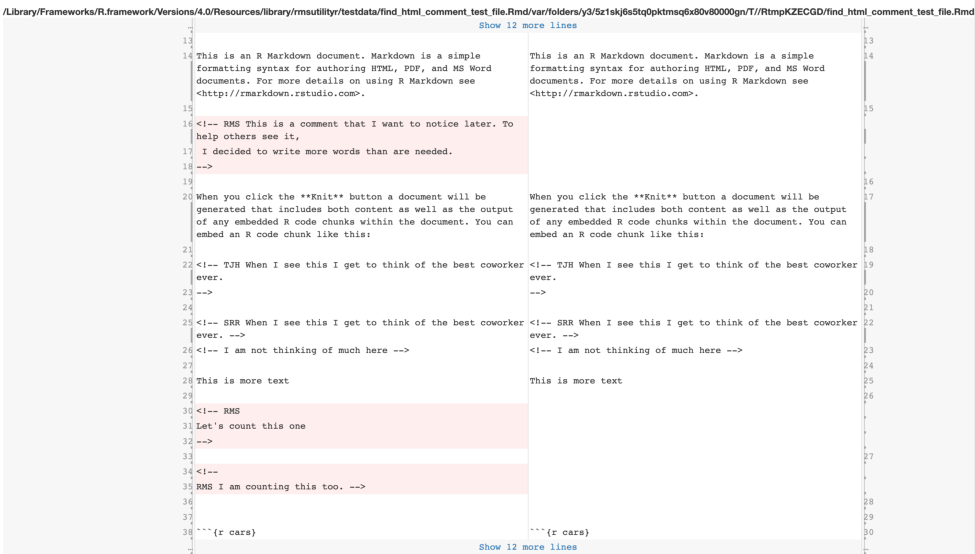
\includegraphics{/Users/msharp/Documents/Development/R/r_workspace/library/rmsutilityr/vignettes/collaborating_with_comments_files/figure-latex/example-diffr-1.pdf}

\end{document}
